\documentclass[UTF8]{ctexart}
\usepackage{xcolor}
% 使用颜色
\definecolor{orange}{RGB}{255,127,0} 
\definecolor{violet}{RGB}{192,0,255} 
\usepackage{geometry}
\setcounter{tocdepth}{5}
\setcounter{secnumdepth}{5}
% 设置四级目录与标题
\geometry{papersize={21cm,29.7cm}}
% 默认大小为A4
\geometry{left=3.18cm,right=3.18cm,top=2.54cm,bottom=2.54cm}
% 默认页边距为1英尺与1.25英尺
\usepackage{indentfirst}
\setlength{\parindent}{2.45em}
% 首行缩进2个中文字符
\usepackage{amssymb}
% 因为所以与其他数学拓展
\usepackage{amsmath}
% 数学公式
\usepackage{setspace}
\renewcommand{\baselinestretch}{1.5}
% 1.5倍行距
\usepackage{pifont}
% 圆圈序号
\usepackage[colorlinks,linkcolor=black,urlcolor=blue]{hyperref}
% 超链接
\usepackage{tikz}
% 绘图
\usepackage{mathtools}
% 有字的长箭头
\author{Didnelpsun}
\title{函数与极限}
\date{}
\begin{document}
\maketitle
\thispagestyle{empty}
\tableofcontents
\thispagestyle{empty}
\newpage
\pagestyle{plain}
\setcounter{page}{1}
\section{邻域}
\subsection{一维}

邻域\textcolor{violet}{\textbf{定义:}}以点$x_0$为中心的任何开区间为点$x_0$的邻域,记为$U(x_0)$。

$\delta$邻域\textcolor{violet}{\textbf{定义:}}设$\delta$为一正数,则称开区间$(x_0-\delta,x_0+\delta)$为点$x_0$的$\delta$邻域,记作$U(x_0,\delta)$。$x_0$称为邻域的中心,$\delta$为邻域的半径。

去心$\delta$邻域就是去除$x_0$的$\delta$邻域,记为$\mathring{U}(x_0,\delta)$,左$\delta$邻域就是左侧的去心$\delta$邻域,记为$U^+(x_0,\delta)$,右$\delta$邻域就是右侧的去心$\delta$邻域,记为$U^-(x_0,\delta)$。

\subsection{二维}

邻域\textcolor{violet}{\textbf{定义:}}设点$P_0(x_0,y_0)$为$xOy$平面上的一点,$\delta$为某一个正数,与点$P_0(x_0,y_0)$的距离小于$\delta$的点$P(x,y)$的全体,称为点$P_0$的$\delta$邻域,记为$U(P_0,\delta)$。

同理可以得到去心$\delta$邻域的定义。

$\delta$邻域的几何意义:以$P_0(x_0,y_0)$为中心,以$\delta>0$为半径的圆内部所有的点。

函数的邻域就是一个区间,所以比如函数在某点的某邻域内有定义,就是说明函数在这个点的附近有定义,这个附近的距离没有必要说明。

\section{定义}

设函数$f(x)$在点$x_0$的某一个去心邻域有定义,若存在常数$A$,对于任意给定的$\epsilon>0$,总存在正数$\delta$,使得当$0<\vert x-x_0\vert<\delta$式,对应的函数值$f(x)$都满足不等式$\vert f(x)-A\vert <\epsilon$,则$A$就是函数$f(x)$当$x\to x_0$时的极限,记作$\lim_{x\to x_0}f(x)=A$或$f(x)\rightarrow A(x\rightarrow x_0)$。

写成$\epsilon-\delta$语言:$\lim_{x\to x_0}f(x)=A\Leftrightarrow\forall\epsilon>0,\exists\delta>0,\text{当}0<\vert x-x_0\vert<\delta$时,有$\vert f(x)-A\vert\epsilon$。

而对于趋向无穷时,写成$\epsilon-X$语言:$\lim_{x\to\infty}f(x)=A\Leftrightarrow\forall\epsilon>0,\exists X>0,\text{当}\vert x\vert>X$时,有$\vert f(x)-A\vert<\epsilon$。

\textcolor{orange}{注意:}这里的趋向分为六种:$x\to x_0$、$x\to x_0^+$、$x\to x_0^-$、$x\to\infty$、$x\to\infty^+$、$x\to\infty^-$。

\subsection{单侧极限}

当$x\to x_0^-$存在的极限称为左极限,当$x\to x_0^+$存在的极限称为右极限。

\subsection{函数极限存在条件}

函数存在的充要条件是:

\begin{enumerate}
    \item $\lim_{x\to x_0}f(x)\Leftrightarrow\lim_{x\to x_0^-}f(x)=\lim_{x\to x_0^+}f(x)=A$。
    \item 函数脱帽法:$\lim_{x\to x_0}f(x)\Leftrightarrow f(x)=A+\alpha(x),\lim_{x\to x_0}\alpha(x)=0$,后面的$\alpha(x)$就是函数与极限值的误差。
\end{enumerate}

\section{性质}

任何$x$的趋向三个性质都是成立的。

\subsection{唯一性}

若极限存在,则极限唯一。

\textbf{例题1:}设$a$为常数,$\lim_{x\to 0}\left(\dfrac{e^{\frac{1}{x}}-\pi}{e^{\frac{2}{x}}+1}+a\cdot\arctan\dfrac{1}{x}\right)$存在,求出极限值。

因为求$x\to 0$,所以需要分两种情况讨论:

$
\begin{aligned}
    & \lim_{x\to 0^+}\left(\dfrac{e^{\frac{1}{x}}-\pi}{e^{\frac{2}{x}}+1}+a\cdot\arctan\dfrac{1}{x}\right) \\
    & = \lim_{x\to 0^+}\left(\dfrac{e^{\frac{1}{x}}-\pi}{e^{\frac{2}{x}}+1}\right)+\lim_{x\to 0^+}\left(a\cdot\arctan\dfrac{1}{x}\right) \\
    & = \lim_{x\to 0^+}\left(\dfrac{0\cdot\left(e^{\frac{2}{x}}\right)^2+e^{\frac{1}{x}}-\pi}{1\cdot\left(e^{\frac{2}{x}}\right)^2+1}\right)+a\cdot\dfrac{\pi}{2} \\
    & = a\cdot\dfrac{\pi}{2} \\
    & \lim_{x\to 0^-}\left(\dfrac{e^{\frac{1}{x}}-\pi}{e^{\frac{2}{x}}+1}+a\cdot\arctan\dfrac{1}{x}\right) \\
    & = -\pi+a\cdot\left(-\dfrac{\pi}{2}\right) \\
    & = -\pi-\dfrac{\pi}{2}\cdot a
\end{aligned}
$

因为极限值具有唯一性,所以$-\pi-\dfrac{\pi}{2}a=\dfrac{\pi}{2}a$,所以$a=-1$,极限值为$-\dfrac{\pi}{2}$。

\subsection{局部有界性}

若极限存在且为$A$,则存在正常数$M$和$\delta$,使得当$0<\vert x-x_0\vert<\delta$时,有$\vert f(x)\vert\leqslant M$。

\begin{enumerate}
    \item 极限存在是函数局部有界性的充分不必要条件。
    \item $f(x)$在$[a,b]$上连续,则$f(x)$在$[a,b]$上有界。
    \item 有限个有界函数与有界函数的和、差、积仍是有界函数。
    \item 若$f'(x)$在有限区间$(a,b)$内有界,则$f(x)$在该区间内有界。
\end{enumerate}

对于结论二,可以利用极限存在必然连续的概念,对$f(x)$在区间两端求极限从而证明有界。这里两端的极限不要求是一样的,因为两端不一样的极限表明该趋向点的极限值不存在,但是仍然有界。

证明结论四:

利用中值定理:$f(b)-f(a)=f'(\xi)(b-a)$。

令$x\in(a,b),x_0\in(a,b)$。其中这两个值不知道大小,只知道范围。

代入中值定理:$f(x)-f(x_0)=f'(\xi)(x-x_0)$

$
\begin{aligned}
    \vert f(x)\vert & =\vert f(x_0)+f'(\xi)(x-x_0)\vert \\
    & \leqslant\vert f(x_0)\vert+\vert f'(\xi)\vert\vert x-x_0\vert\text{ (重要绝对值不等式)} \\
    & \leqslant\vert f(x_0)\vert+K\cdot(b-a) \\
    & \leqslant M
\end{aligned}
$

\textbf{例题2:}函数$f(x)=\dfrac{\vert x\vert\sin(x-2)}{x(x-1)(x-2)^2}$在哪个区间内有界()。

$A.(-1,0)$\qquad$B.(0,1)$\qquad$C.(1,2)$\qquad$D.(2,3)$

解:看选项,0,1,2出现次数较多,所以从$B$选项开始检查是否有界:

$\lim_{x\to 0^-}\dfrac{\vert x\vert\sin(x-2)}{x(x-1)(x-2)^2}=(-1)\cdot\dfrac{-\sin 2}{(-1)\cdot 4}=-\dfrac{\sin 2}{4}$

所以趋于$0^-$的一段有界。

同理$\lim_{x\to 0^+}\dfrac{\vert x\vert\sin(x-2)}{x(x-1)(x-2)^2}=\dfrac{\sin 2}{4}$。

所以趋于$0^+$的一段有界。

$\lim_{x\to 1^-}\dfrac{\vert x\vert\sin(x-2)}{x(x-1)(x-2)^2}$中$(x-1)$为0且在分母位置,所以极限为$\infty$,无界。

所以$(0,1)$无界,$B$排除。

同理$\lim_{x\to 1^+}\dfrac{\vert x\vert\sin(x-2)}{x(x-1)(x-2)^2}$也无穷大而无界。

所以$(1,2)$无界,$C$排除。

$\lim_{x\to 2^+}\dfrac{\vert x\vert\sin(x-2)}{x(x-1)(x-2)^2}$中不管前面的项,而看到后面的$\dfrac{\sin(x-2)}{(x-2)^2}$。

因为$\lim_{x\to 0}\dfrac{\sin x}{x}=1$,所以对于$\lim_{x\to 2}\dfrac{\sin(x-2)}{(x-2)}=1$,所以下面还有一个$x-2$,所以还是为$\infty$。

所以$(2,3)$无界,$D$排除。

验证-1处是否有界:

$\lim_{x\to -1}\dfrac{\vert x\vert\sin(x-2)}{x(x-1)(x-2)^2}=-\dfrac{\sin 3}{18}$。

所以该处有界,所以选$A$。

\subsection{局部保号性}

若极限存在,则存在常数$\delta>0$,使得当$0<\vert x-x_0\vert<\delta$时,$f(x)$与$A$同号。

简单来说,函数值在$x\to x_0$时函数值与极限值同号。

证明局部保号性:

首先根据极限存在定义:$\forall\epsilon>0,\exists\delta>0,0<\vert x-x_0\vert<\delta$时,恒有$\vert f(x)-A\vert<\epsilon$。

$\Rightarrow -\epsilon<f(x)-A<\epsilon$

$\Rightarrow A-\epsilon<f(x)<A+\epsilon$

任意取$\epsilon=\dfrac{A}{2}>0\Rightarrow f(x)>A-\dfrac{A}{2}=\dfrac{A}{2}>0$

证明完毕。

关于$\epsilon$的取值问题,为什么不能取到令结果为负的值,因为请注意这个取值得到的区间并不是$f(x)$的范围,而是对$f(x)$所在区间的陈述,其是无尽逼近$A$的,所以取多大的区间都无所谓。

推论:若函数值在$x\to x_0$时都非负或非正,极限值为$A$,那么$A$与此时函数值同号。不能去除等号。

\bigskip

关于三个性质要注意自变量取值的双向性,所以需要留意下面几个函数:

\begin{enumerate}
    \item $\lim_{x\to\infty}e^x$不存在,因为$\lim_{x\to +\infty}e^x=+\infty$,$\lim_{x\to -\infty}e^x=0$。
    \item $\lim_{x\to 0}\dfrac{\sin x}{\vert x\vert}$不存在,因为$\lim_{x\to 0^+}\dfrac{\sin x}{\vert x\vert}=1$,$\lim_{x\to 0^-}\dfrac{\sin x}{\vert x\vert}=-1$。
    \item $\lim_{x\to\infty}\arctan x$不存在,因为$\lim_{x\to +\infty}\arctan x=\dfrac{\pi}{2}$,$\lim_{x\to -\infty}\arctan x=-\dfrac{\pi}{2}$。
    \item $\lim_{x\to 0}[x]$不存在,因为$\lim_{x\to 0^+}[x]=0$,$\lim_{x\to 0^-}[x]=-1$
\end{enumerate}

\section{运算法则}

若$\lim f(x)=A$,$\lim g(x)=B$,则

\begin{enumerate}
    \item $\lim[k\cdot f(x)\pm l\cdot g(x)]=k\lim f(x)\pm l\cdot g(x)=kA\pm lB$,其中$kl$为常数。
    \item $\lim[f(x)\cdot g(x)]=\lim f(x)\cdot\lim g(x)=A\cdot B$
    \item $\lim[f(x)]^n=[\lim f(x)]^n$,其中$n$为正整数。
    \item $\lim\dfrac{f(x)}{g(x)}=\dfrac{\lim f(x)}{\lim g(x)}=\dfrac{A}{B}(B\neq 0)$。
\end{enumerate}

\section{夹逼准则}

\begin{enumerate}
    \item $g(x)\leqslant f(x)\leqslant h(x)$。
    \item $\lim g(x)=A$且$\lim h(x)=A$。
    \item 则$\lim f(x)=A$。
\end{enumerate}

\textcolor{orange}{注意:}两函数差值极限为0不代表两函数极限相同,也不能保证中间的$f(x)$的极限存在。

\section{洛必达法则}

\textcolor{aqua}{\textbf{定理:}}

\begin{enumerate}
    \item 当$x\to a\text{或}\infty$时,函数$f(x)$,$g(x)$都趋向0或无穷大。
    \item $f'(x)$和$F'(x)$在点$a$的某去心邻域内,或$\vert x\vert$大于充分大的正数时,存在,且$g'(x)\neq 0$。
    \item $\lim_{x\to a}\dfrac{f'(x)}{g'(x)}$或$\lim_{x\to\infty}\dfrac{f'(x)}{g'(x)}$存在或无穷大。
    \item $\lim_{x\to a}\dfrac{f(x)}{g(x)}=\lim_{x\to a}\dfrac{f'(x)}{g'(x)}$或$\lim_{x\to\infty}\dfrac{f(x)}{g(x)}=\lim_{x\to\infty}\dfrac{f'(x)}{g'(x)}$。
\end{enumerate}

\textcolor{orange}{注意:}

\begin{enumerate}
    \item 如果函数比值不为$\dfrac{0}{0}$或$\dfrac{\infty}{\infty}$型,则不能使用洛必达法则。
    \item 若求导后极限仍为$\dfrac{0}{0}$或$\dfrac{\infty}{\infty}$型,则可以继续使用洛必达法则。
    \item 若$\lim_{x\to a}\dfrac{f'(x)}{g'(x)}$不存在且不为$\infty$,不能反推$\lim_{x\to a}\dfrac{f(x)}{g(x)}$不存在也不为$\infty$,这时候洛必达法则是失效的。
\end{enumerate}

对于第三个注意点:$\lim_{x\to 0}\dfrac{x^2\cdot\sin\dfrac{1}{x}}{x}=\lim_{x\to 0}x\cdot\sin\dfrac{1}{x}=0$。

而使用洛必达法则:

$\lim_{x\to 0}\dfrac{x^2\cdot\sin\dfrac{1}{x}}{x}=\lim_{x\to 0}\left(2x\cdot\sin\dfrac{1}{x}-\cos\dfrac{1}{x}\right)=\lim_{x\to 0}\left(-\cos\dfrac{1}{x}\right)=\text{不存在}$。

\section{泰勒公式}

非常重要。

\subsection{定义}

是一个用函数在某点的信息描述其附近取值的公式。如果函数满足一定的条件,泰勒公式可以用函数在某一点的各阶导数值做系数构建一个多项式来近似表达这个函数。即形式:$f(x)=\sum ax^n$。

简单来说,泰勒公式就是一个近似表达函数的公式。其极限趋向为趋向0。

对于泰勒公式以及后面的中值定理等相关延申见\href{https://www.zhihu.com/question/25627482}{知乎回答}。

\subsection{泰勒展开}

当$x\to 0$时:

\begin{enumerate}
    \item $\sin x=x-\dfrac{x^3}{3!}+o(x^3)$。
    \item $\cos x=1-\dfrac{x^2}{2!}+\dfrac{x^4}{4!}+o(x^4)$。
    \item $\arcsin x=x+\dfrac{x^3}{3!}+o(x^3)$。
    \item $\tan x=x+\dfrac{x^3}{3}+o(x^3)$。
    \item $\arctan x=x-\dfrac{x^3}{3}+o(x^3)$。
    \item $\ln(1+x)=x-\dfrac{x^2}{2}+\dfrac{x^3}{3}+o(x^3)$。
    \item $e^x=1+x+\dfrac{x^2}{2!}+\dfrac{x^3}{3!}+o(x^3)$。
    \item $(1+x)^\alpha=1+\alpha\cdot x+\dfrac{\alpha\cdot(\alpha-1)}{2!}x^2+o(x^2)$。
\end{enumerate}

其中$o(x^\alpha)$为佩亚诺余项,其非常小。

同样可以对泰勒展开式进行变形:$x-\sin x\sim\dfrac{x^3}{6}$,$x+\sin x\sim 2x$。

如:

$
\begin{aligned}
    & \lim_{x\to 0}\dfrac{[\sin x-\sin(\sin x)]\sin x}{x^4} \\
    & =\dfrac{\dfrac{1}{6}\sin^3x\cdot\sin x}{x^4} \\
    & =\dfrac{\dfrac{1}{6}\sin^4x}{x^4} \\
    & =\dfrac{1}{6}
\end{aligned}
$

\subsection{无穷小运算}

\begin{enumerate}
    \item 有限个无穷小的和是无穷小。
    \item 有界函数与无穷小的乘积是无穷小。
    \item 有限个无穷小的乘积是无穷小。
\end{enumerate}

无穷小运算,设$m$,$n$为正整数:

\begin{enumerate}
    \item $o(x^m)\pm o(x^n)=o(x^l),l=\min{m,n}$(加减法低阶吸收高阶)。
    \item $o(x^m)\cdot o(x^n)=o(x^{m+n}),x^m\cdot o(x^n)=o(x^{m+n})$(乘法累加)。
    \item $o(x^m)=o(k\cdot x^m)=k\cdot o(x^m)$,$k\neq 0$且为常数(非零常数相乘不影响阶数)。
\end{enumerate}

\subsection{展开幂的选择}

泰勒公式展开时应该展开到多少次幂?

\subsubsection{\texorpdfstring{$\dfrac{A}{B}$}型,上下同阶}

当分母或分子式$x$的$k$次幂那么应该把分母或分子展开到对应的次数幂。

如$\lim_{x\to 0}\dfrac{x-\sin x}{x^3}$展开为三次:

$
\begin{aligned}
    & \lim_{x\to 0}\dfrac{x-\sin x}{x^3} \\
    & =\lim_{x\to 0}\dfrac{x-\left[x-\dfrac{1}{6}x^3+o(x^3)\right]}{x^3} \\
    & =\lim_{x\to 0}\dfrac{\dfrac{1}{6}x^3+o(x^3)}{x^3} \\
    & =\dfrac{1}{6}
\end{aligned}
$

\subsubsection{\texorpdfstring{$A-B$}型,幂次最低}

将$A$,$B$分别展到他们系数不相等的$x$的最低次幂为止。

如已知当$x\to 0$时,$\cos x-e^{-\frac{x^2}{2}}$与$ax^k$为等价无穷小,求$a$,$b$。

泰勒展开:

$
\begin{aligned}
    & \cos x-e^{-\frac{x^2}{2}} \\
    & = 1-\dfrac{x^2}{2}+\dfrac{1}{24}x^4+o(x^4)-\left(1-\dfrac{x^2}{2}+\dfrac{1}{8}x^4+o(x^4)\right) \\
    & = -\dfrac{1}{12}x^4+o(x^4) \\
    & \sim -\dfrac{1}{12}x^4
\end{aligned}
$

$\therefore a=-\dfrac{1}{12},b=4$。

\textbf{例题3:}求解$\lim_{x\to 0}\dfrac{\sin^2x-x^2}{e^{x^4}-1}$。

首先由泰勒展开式$e^x=1+x+o(x)$,得到$e^x-1\sim x$。

$\therefore e^{x^4}-1\sim x^4$。

然后泰勒展开:

$
\begin{aligned}
    & x-\sin x \\
    & = 1\cdot x^1+0\cdot x^3 - (1\cdot x^1-\dfrac{1}{6}x^3+o(x^3)) \\
    & = \dfrac{1}{6}x^3+o(x^3) \\
    & \sim \dfrac{1}{6}x^3
\end{aligned}
$

$
\begin{aligned}
    & x+\sin x \\
    & =x-(-\sin x) \\
    & =1\cdot x^1-(-1\cdot x^1)+o(x) \\
    & =2x+o(x) \\
    & \sim 2x
\end{aligned}
$

$\therefore$ \bigskip

$
\begin{aligned}
    & \lim_{x\to 0}\dfrac{\sin^2x-x^2}{e^{x^4}-1} \\
    & =\lim_{x\to 0}\dfrac{(\sin x+x)(\sin x-x)}{x^4} \\
    & =\lim_{x\to 0}\dfrac{2x\cdot\left(-\dfrac{1}{6}x^3\right)}{x^4} \\
    & =-\dfrac{1}{3}
\end{aligned}
$

\section{海涅定理(归结原则)}

\subsection{定义}

设$f(x)$在$\mathring{U}(x_0,\delta)$内有定义,则$\lim_{x\to x_0}f(x)=A$存在$\Leftrightarrow$对任何$\mathring{U}(x_0,\delta)$内以$x_0$为极限的数列$\{x_n\}(x_n\neq x_0)$,极限$\lim_{n\to\infty}f(x_n)=A$存在。

海涅定理用来连接数列极限与函数极限。在极限存在下他们可以相互转换。

\textbf{例题4:}求$\lim_{n\to\infty}\left(n\tan\dfrac{1}{n}\right)^{n^2}$($n\in N^+$)。

$\because \lim_{x\to 0}\left(\dfrac{\tan x}{x}\right)^{\frac{1}{x^2}}$

又$u^v=e^{v\ln u}$

$\therefore =e^{\lim_{x\to 0}\frac{1}{x^2}\ln\frac{\tan x}{x}}$

又在$x\to 0$下$\ln (1+x)\sim x$,$\therefore \ln(1+g(x))\sim g(x),g(x)\to 0$。

而$\dfrac{\tan x}{x}$在$x\to 0$时趋于1,不满足趋于0的条件,所以正好变形$\ln\left(1+\dfrac{\tan x}{x}-1\right)$。

$\therefore \ln\left(1+\dfrac{\tan x}{x}-1\right)\sim\dfrac{\tan x}{x}-1$,$\dfrac{\tan x}{x}-1\to 0$。

又泰勒展开$\tan x-x=x+\dfrac{x^3}{3}+o(x^3)-x-0\cdot x^3=\dfrac{x^3}{3}$。

$\therefore$ \bigskip

$
\begin{aligned}
    & e^{\lim_{x\to 0}\frac{1}{x^2}\ln\frac{\tan x}{x}} \\
    & =e^{\lim_{x\to 0}\frac{1}{x^2}\frac{\tan x-x}{x}} \\
    & =e^{\lim_{x\to 0}\frac{1}{x^2}\cdot\frac{x^2}{3}} \\
    & = e^{\frac{1}{3}}
\end{aligned}
$

根据海涅定理:取$x=\dfrac{1}{n},n\to\infty$,$\lim_{n\to\infty}\left(n\tan\dfrac{1}{n}\right)^{n^2}=e^{\frac{1}{3}}$。

\section{无穷小比阶}

\subsection{无穷定义}

当$x\to x_0(\infty)$时,函数$f(x)$极限为0,就称$f(x)$为当$x\to x_0(\infty)$时的无穷小,记为:$\lim_{x\to x_0(\infty)}f(x)=0$。

以0为极限的数列称为$n\to\infty$时的无穷小。

无穷大\textcolor{violet}{\textbf{定义:}}当$x\to x_0(\infty)$时,函数$\vert f(x)\vert$无限增大,就称$f(x)$为当$x\to x_0(\infty)$时的无穷大,记为:$\lim_{x\to x_0(\infty)}f(x)=\infty$。

\subsection{无穷小比阶定义}

设在自变量同一变化过程中,$\lim\alpha(x)=0$,$\lim\beta(x)=0$,且$\beta(x)\neq 0$,则:

\begin{enumerate}
    \item 若$\lim\dfrac{\alpha(x)}{\beta(x)}=0$,则$\alpha(x)$是比$\beta(x)$高阶的无穷小,记为$\alpha(x)=o(\beta(x))$。
    \item 若$\lim\dfrac{\alpha(x)}{\beta(x)}=\infty$,则$\alpha(x)$是比$\beta(x)$低阶的无穷小。
    \item 若$\lim\dfrac{\alpha(x)}{\beta(x)}=c\neq 0$,则$\alpha(x)$与$\beta(x)$是同阶无穷小。
    \item 若$\lim\dfrac{\alpha(x)}{\beta(x)}=1$,则$\alpha(x)$与$\beta(x)$是等价无穷小,记为$\alpha(x)\sim\beta(x)$。
    \item 若$\lim\dfrac{\alpha(x)}{[\beta(x)]^k}=c\neq 0$,则$\alpha(x)$是$\beta(x)$的$k$阶无穷小。
\end{enumerate}

并不是任意无穷小都可以比阶。如$\lim_{x\to 0}\dfrac{x\sin\dfrac{1}{x}}{x^2}$就因为得到函数振荡而无法得到极限。

\subsection{常用等价无穷小}

$x\to 0$:

\begin{enumerate}
    \item $\sin x\sim x$。
    \item $\tan x\sim x$。
    \item $\arcsin x\sim x$。
    \item $\arctan x\sim x$。
    \item $\ln(1+x)\sim x$。
    \item $e^x-1\sim x$。
    \item $a^x-1\sim x\ln a$。
    \item $1-\cos x\sim\dfrac{1}{2}x^2$。
    \item $(1+x)^a-1\sim ax$。
\end{enumerate}

还有$e^{\sin x}-e^x\sim\sin x-x\sim-\dfrac{1}{6}x^3$。

其中$a\cdot x\ln x$当$x\to 0$的极限必然为0。

\section{极限计算}

\subsection{未定式}

未定式即需要自己定义的式子,可能存在极限也可能不存在,对于自变量的变化趋势分为六种,分别是对于$x_0$与$\infty$的各三种。

\subsubsection{化简}

方式:

\begin{enumerate}
    \item 提出极限不为0的因式。
    \item 等价无穷小替换。
    \item 恒等变形(提公因式、拆项、合并、分子分母同除变量最高次幂、换元法)。
\end{enumerate}

\subsubsection{判断类型}

七种:$\dfrac{0}{0},\dfrac{\infty}{\infty},0\cdot\infty,\infty-\infty,\infty^0,0^0,1^\infty$。

\ding{172}其中$\dfrac{0}{0}$为洛必达法则的基本型。$\dfrac{\infty}{\infty}$可以类比$\dfrac{0}{0}$的处理方式。$0\cdot\infty$可以转为$\dfrac{0}{\dfrac{1}{\infty}}=\dfrac{0}{0}=\dfrac{\infty}{\dfrac{1}{0}}=\dfrac{\infty}{\infty}$。设置分母有原则,简单因式才下放。(简单:幂函数,e为底的指数函数)

\ding{173}$\infty-\infty$可以提取公因式或通分,即和差化积。

\ding{174}$\infty^0,0^0,1^\infty$,就是幂指函数。

$
u^v=e^{v\ln u}=\left\{
\begin{array}{lcl}
    \infty^0 & \rightarrow & e^{0\cdot+\infty} \\
    0^0 & \rightarrow & e^{0\cdot-\infty} \\
    1^\infty & \rightarrow & e^{\infty\cdot 0} \\
\end{array} \right.
$

$\therefore \lim u^v=e^{\lim v\cdot\ln u}=e^{\lim v(u-1)}$

\paragraph{比值类型} \leavevmode \bigskip

$\dfrac{0}{0}$型\textbf{例题5:}求极限$\lim_{x\to 0}\dfrac{e^{-\frac{1}{x^2}}}{x^{100}}$

$
\begin{aligned}
    & \lim_{x\to 0}\dfrac{e^{-\frac{1}{x^2}}}{x^{100}} \\
    & = \lim_{x\to 0}\dfrac{e^{-\frac{1}{x^2}}\cdot 2x^{-3}}{100x^99} \\
    & = \lim_{x\to 0}\dfrac{1}{50}\lim_{x\to 0}\dfrac{e^{-\frac{1}{x^2}}}{x^{102}}
\end{aligned}
$

\bigskip

使用洛必达法则下更复杂,因为分子的幂次为负数,导致求导后幂次绝对值越来越大,不容易计算。

使用倒代换再洛必达降低幂次,令$\dfrac{1}{x^2}=t$。

$
\begin{aligned}
    & \lim_{x\to 0}\dfrac{e^{-\frac{1}{x^2}}}{x^{100}} \\
    & = \lim_{t\to+\infty}\dfrac{e^{-t}}{t^{-50}} \\
    & = \lim_{t\to+\infty}\dfrac{t^{50}}{e^t} \\
    & = \lim_{t\to+\infty}\dfrac{50t^{49}}{e^t} \\
    & = \cdots \\
    & = \lim_{t\to+\infty}\dfrac{50!}{e^t} \\
    & = 0
\end{aligned}
$

$\infty\cdot 0$型\textbf{例题6:}求极限$\lim_{x\to-\infty}x(\sqrt{x^2+100}+x)$。

首先定性分析:$\lim_{x\to-\infty}x\cdot(\sqrt{x^2+100}+x)$。

在$x\to-\infty$趋向时,$x$就趋向无穷大,而$\sqrt{x^2+100}$为一次,所以$\sqrt{x^2+100}+x$趋向0。

又$\sqrt{x^2+100}$在$x\to-\infty$时本质为根号差,所以有理化:

$
\begin{aligned}
    & \lim_{x\to-\infty}x(\sqrt{x^2+100}+x) \\
    & \lim_{x\to-\infty}x\dfrac{x^2+100-x^2}{\sqrt{x^100}-x} \\
    & = \lim_{x\to-\infty}\dfrac{100x}{\sqrt{x^2+100}-x} \\
    & \xRightarrow{\text{令}x=-t}\lim_{t\to+\infty}\dfrac{-100t}{\sqrt{t^2+100}+t} \\
    & = \lim_{t\to+\infty}\dfrac{-100}{\sqrt{1+\dfrac{100}{t^2}}+1} \\
    & = -50
\end{aligned}
$

$\infty\cdot 0$型\textbf{例题7:}求极限$\lim_{x\to 1^-}\ln x\ln(1-x)$。

当$x\to 1^-$时,$\ln x$趋向0,$\ln(1-x)$趋向$-\infty$。

又$x\to 0$,$\ln(1+x)\sim x$,所以$x\to 1$,$\ln x\sim x-1$:

$
\begin{aligned}
    & \lim_{x\to 1^-}\ln x\ln(1-x) \\
    & = \lim_{x\to 1^-}(x-1)\ln(1-x) \\
    & \xRightarrow{令t=1-x} =-\lim_{t\to 0^+}t\ln t \\
    & = -\lim_{t\to 0^+}\dfrac{\ln t}{\dfrac{1}{t}} \\
    & = -\lim_{t\to 0^+}\dfrac{\dfrac{1}{t}}{-\dfrac{1}{t^2}} \\
    & = \lim_{t\to 0^+}t \\
    & = 0
\end{aligned}
$


$\dfrac{0}{0}$型\textbf{例题8:}求极限$\lim_{x\to 0}\dfrac{\arcsin x-\arctan x}{\sin x-\tan x}$。

分析:该题目使用洛必达法则会比较麻烦且难以计算,所以先考虑是否能用泰勒展开:

$x\to 0$,$\sin x=x-\dfrac{1}{6}x^3+o(x^3)$,$\tan x=x+\dfrac{1}{3}x^3+o(x^3)$,$\arcsin x=x+\dfrac{1}{6}x^3+o(x^3)$,$\arctan x=x-\dfrac{1}{3}x^3+o(x^3)$。

$\therefore \sin x-\tan x=-\dfrac{1}{2}x^3+o(x^3)$,$\arcsin x-\arctan x=\dfrac{1}{2}x^3+o(x^3)$

$\therefore \text{原式}=\dfrac{\dfrac{1}{x}x^3+o(x^3)}{-\dfrac{1}{2}x^3+o(x^3)}=-1$。

$0\cdot\infty$型\textbf{例题9:}求极限$\lim_{x\to 0}x\left[\dfrac{10}{x}\right]$,其中$[\cdot]$为取整符号。

取整函数公式:$x-1<[x]\leqslant x$,所以$\dfrac{10}{x}-1<\left[\dfrac{10}{x}\right]\leqslant\dfrac{10}{x}$。

当$x>0$时,$x\to 0^+$,两边都乘以10,$10-x<x\cdot\left[\dfrac{10}{x}\right]\leqslant x\cdots\dfrac{10}{x}=10$,而左边在$x\to 0^+$时极限也为10,所以夹逼准则,中间$x\cdot\left[\dfrac{10}{x}\right]$极限也为10。

当$x>0$时,$x\to 0^-$,同样也是夹逼准则得到极限为10。

$\therefore \lim_{x\to 0}x\left[\dfrac{10}{x}\right]$。

\paragraph{差类型} \leavevmode \bigskip

\begin{itemize}
    \item 如果函数中有分母,则通分,将加减法变形为乘除法,以便其他计算如洛必达法则。
    \item 若函数中没有分母,则可以通过提取公因式或倒数代换,出现分母,再利用通分等方式将加减法变成乘除法。
\end{itemize}

$\infty-\infty$型\textbf{例题10:}求极限$\lim_{x\to 0}\left(\dfrac{1}{\sin^2x}-\dfrac{\cos^2x}{x^2}\right)$。

$
\begin{aligned}
    & \lim_{x\to 0}\left(\dfrac{1}{\sin^2x}-\dfrac{\cos^2x}{x^2}\right) \\
    & = \lim_{x\to 0}\dfrac{x^2-\sin^2x\cos^2x}{\sin^2x\cdot x^2} (\sin x\sim x)\\
    & = \lim_{x\to 0}\dfrac{x^2-\sin^2x\cos^2x}{x^4} (\sin x\cos x\sim\dfrac{1}{2}\sin 2x)\\
    & = \lim_{x\to 0}\dfrac{x^2-\dfrac{1}{4}\sin^22x}{x^4} \\
    & = \lim_{x\to 0}\dfrac{2x-\dfrac{1}{4}\cdot 2\sin 2x\cdot\cos 2x\cdot 2}{4x^3} (\sin x\cos x\sim\dfrac{1}{2}\sin 2x)\\
    & = \lim_{x\to 0}\dfrac{2x-\dfrac{1}{2}\sin 4x}{4x^3} \\
    & = \lim_{x\to 0}\dfrac{2-\dfrac{1}{2}\cos 4x\cdot 4}{12x^2} \\
    & = \dfrac{1}{6}\lim_{x\to 0}\dfrac{1-\cos 4x}{x^2} (1-\cos x\sim \dfrac{1}{2}x^2)\\
    & = \dfrac{4}{3}
\end{aligned}
$

$\infty-\infty$型\textbf{例题11:}求极限$\lim_{x\to+\infty}[x^2(e^{\frac{1}{x}}-1)-x]$。

该式子无法进行因式分解,所以尝试使用倒数代换:

$
\begin{aligned}
    & \lim_{x\to+\infty}[x^2(e^{\frac{1}{x}}-1)-x] \\
    & \xRightarrow{\text{令}x=\frac{1}{t}}\lim_{t\to 0^+}\left(\dfrac{e^t-1}{x^2}-\dfrac{1}{t}\right) \\
    & \lim_{t\to 0^+}\dfrac{e^t-1-t}{t^2} \\
    & \xRightarrow{\text{泰勒展开}e^x}\lim_{t\to 0^+}\dfrac{\dfrac{1}{2}x^2}{x^2} \\
    & =\dfrac{1}{2}
\end{aligned}
$

\paragraph{幂指类型} \leavevmode \bigskip

$\infty^0$型\textbf{例题12:}求极限$\lim_{x\to+\infty}(x+\sqrt{1+x^2})^{\frac{1}{x}}$。

$
\begin{aligned}
    & \lim_{x\to+\infty}(x+\sqrt{1+x^2})^{\frac{1}{x}} \\
    & =e^{\lim_{x\to+\infty}\frac{(x+\sqrt{1+x^2})}{x}} \left(\ln(x+\sqrt{1+x^2})'=\dfrac{1}{\sqrt{1+x^2}}\right) \\
    & =e^{\lim_{x\to+\infty}\dfrac{1}{\sqrt{1+x^2}}} \\
    & =e^0 \\
    & =1
\end{aligned}
$

$1^\infty$型\textbf{例题13:}求极限$\lim_{x\to 0}\left(\dfrac{e^x+e^{2x}+\cdots+e^{nx}}{n}\right)^{\frac{e}{x}}$。($n\in N^+$)

$
\begin{aligned}
    & \lim_{x\to 0}\left(\dfrac{e^x+e^{2x}+\cdots+e^{nx}}{n}\right)^{\frac{e}{x}} \\
    & =e^{\lim_{x\to 0}\dfrac{e}{x}\ln\left(\frac{e^x+e^{2x}+\cdots+e^{nx}}{n}\right)} \\
    & =e^{\lim_{x\to 0}\dfrac{e}{x}\left(\frac{e^x+e^{2x}+\cdots+e^{nx}}{n}-1\right)} \\
    & =e^{\lim_{x\to 0}\dfrac{e}{x}\left(\frac{e^x+e^{2x}+\cdots+e^{nx}-n}{n}\right)} \\
    & =e^{\frac{e}{n}\lim_{x\to 0}\left(\frac{e^x-1}{x}+\frac{e^{2x}-1}{x}+\cdots+\frac{e^{nx}-1}{x}\right)} \\
    & =e^{\frac{e}{n}[1+2+\cdots+n]} \\
    & =e^{\frac{e}{n}\cdot\frac{n(1+n)}{2}} \\
    & =e^{\frac{e(1+n)}{2}}
\end{aligned}
$

\subsection{极限转换}

一般解法为两种,一种是脱帽法:$\lim_{x\to x_0}f(x)\Leftrightarrow f(x)=A+\alpha(x),\lim_{x\to x_0}\alpha(x)=0$。第二种就是根据之间的关系转换。

\textbf{例题14:}如果$\lim_{x\to 0}\dfrac{x-\sin x+f(x)}{x^4}$存在,则$\lim_{x\to 0}\dfrac{x^3}{f(x)}$为常数多少?

解法一:

由$\lim_{x\to 0}\dfrac{x\sin x+f(x)}{x^4}=A$脱帽:$\dfrac{x\sin x+f(x)}{x^4}=A+\alpha$。

得到:$f(x)=Ax^4+\alpha\cdot x^4-(x-\sin x)$。

反代入:$\lim_{x\to 0}\dfrac{f(x)}{x^3}=\lim_{x\to 0}\dfrac{Ax^4+\alpha\cdot x^4-x+\sin x}{x^3}=0+0-\dfrac{1}{6}=-\dfrac{1}{6}$。

$\therefore \lim_{x\to 0}\dfrac{x^3}{f(x)}=-6$。

解法二:

由$\lim_{x\to 0}\dfrac{x\sin x+f(x)}{x^4}=A$,而目标是$x^3$,所以需要变形:

$
\begin{aligned}
    & \lim_{x\to 0}\dfrac{x\sin x+f(x)}{x^4}=A \\
    & \lim_{x\to 0}\dfrac{x\sin x+f(x)\cdot x}{x^4}=A\cdot\lim_{x\to 0}x=0 \\
    & \lim_{x\to 0}\dfrac{x-\sin x}{x^3}+\lim_{x\to 0}\dfrac{f(x)}{x^3}=0 \\
    & \text{泰勒展开:}x-\sin x=\dfrac{1}{6}x^3 \\
    & \lim_{x\to 0}\dfrac{f(x)}{x^3}=-\dfrac{1}{6} \\
    & \lim_{x\to 0}\dfrac{x^3}{f(x)}=-6
\end{aligned}
$

\subsection{求参数}

因为求参数类型的题目中式子是未知的,所以求导后也是未知的,所以一般不要使用洛必达法则,而使用泰勒展开。

一般极限式子右侧等于一个常数,或是表明高阶或低阶。具体的关系参考无穷小比阶。

\textbf{例题15:}设$\lim_{x\to 0}\dfrac{\ln(1+x)-(ax+bx^2)}{x^2}=2$,求常数a,b。

根据泰勒展开式:$x\to 0,\ln(1+x)=x-\dfrac{x^2}{x}+o(x^2)$。

$
\begin{aligned}
    & \lim_{x\to 0}\dfrac{\ln(1+x)-(ax+bx^2)}{x^2}=2 \\
    & =\lim_{x\to 0}\dfrac{(1-a)x-\left(\dfrac{1}{2}+b\right)x^2+o(x^2)}{x^2}=2\neq 0 \\
    & 1-a=0;-\left(\dfrac{1}{2}+b\right)=2 \\
    & \therefore a=1;b=-\dfrac{5}{2}
\end{aligned}
$

\textcolor{orange}{注意:}根据泰勒公式,$x-\ln(1+x)\sim\dfrac{1}{2}x^2\sim 1-\cos x$。

函数的连续与间断是逐点的概念。

\section{连续}
\subsection{定义}

若函数$f(x)$在点$x_0$的某一邻域内有定义,且有$\lim_{x\to x_0}f(x)=f(x_0)$,则称函数$f(x)$在点$x_0$处连续。

极限值等于函数值,则该点连续。

\section{间断}

讨论间断只看两类点:分段函数分段点,无定义点。

\subsection{定义}

若函数$f(x)$在点$x_0$的某一去心邻域内有定义,且有$\lim_{x\to x_0}f(x)\neq f(x_0)$,则称函数$f(x)$在点$x_0$处间断。

极限值不等于函数值,则该点间断。

\subsection{分类}
\subsubsection{可去间断点(可补间断点)}

若$\lim_{x\to x_0}f(x)=A\neq f(x_0)$(甚至可以没有定义)。

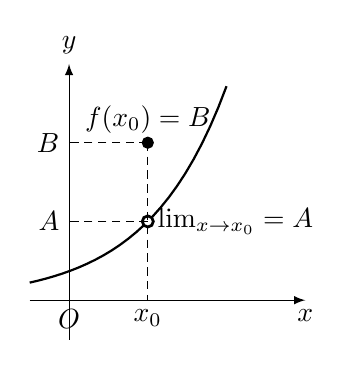
\begin{tikzpicture}
    \draw[-latex](-0.5,0) -- (3,0) node[below]{$x$};
    \draw[-latex](0,-0.5) -- (0,3) node[above]{$y$};
    \filldraw[black] (0,0) node[below]{$O$};
    \draw[black, thick, domain=-0.5:2] plot (\x,{pow(e,\x-1)});
    \filldraw[white, draw=black, line width=1pt] (1,1) circle (2pt);
    \draw[black, densely dashed](1,2) -- (0,2) node[left]{$B$};
    \draw[black, densely dashed](1,1) -- (0,1) node[left]{$A$};
    \draw[black, densely dashed](1,2) -- (1,0) node[below]{$x_0$};
    \filldraw[black] (1,2) circle (2pt) node[above]{$f(x_0)=B$};
    \filldraw[black] (1,1) node[right]{$\lim_{x\to x_0}=A$};
\end{tikzpicture}

\subsubsection{跳跃间断点}

若$\lim_{x\to x_0^-}f(x)$与$\lim_{x\to x_0^+}$都存在,但是$\lim_{x\to x_0^-}f(x)\neq\lim_{x\to x_0^+}$。

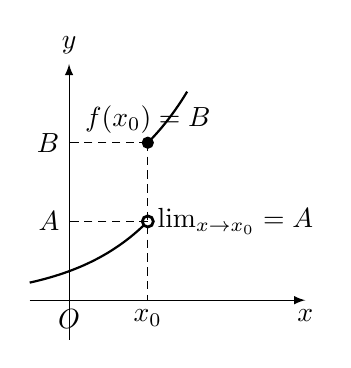
\begin{tikzpicture}
    \draw[-latex](-0.5,0) -- (3,0) node[below]{$x$};
    \draw[-latex](0,-0.5) -- (0,3) node[above]{$y$};
    \filldraw[black] (0,0) node[below]{$O$};
    \draw[black, thick, domain=-0.5:1] plot (\x,{pow(e,\x-1)});
    \draw[black, thick, domain=1:1.5] plot (\x,{pow(e,\x-1)+1});
    \filldraw[white, draw=black, line width=1pt] (1,1) circle (2pt);
    \draw[black, densely dashed](1,2) -- (0,2) node[left]{$B$};
    \draw[black, densely dashed](1,1) -- (0,1) node[left]{$A$};
    \draw[black, densely dashed](1,2) -- (1,0) node[below]{$x_0$};
    \filldraw[black] (1,2) circle (2pt) node[above]{$f(x_0)=B$};
    \filldraw[black] (1,1) node[right]{$\lim_{x\to x_0}=A$};
\end{tikzpicture}

可去间断点与跳跃间断点都称为第一类间断点。

\subsubsection{无穷间断点}

若$\lim_{x\to x_0}f(x)=\infty$,或至少一个方向为无穷大(定义分歧)。如$y=\dfrac{1}{x}$在$x=0$处为无穷间断点。

\begin{tikzpicture}
    \draw[-latex](-2,0) -- (2,0) node[below]{$x$};
    \draw[-latex](0,-2) -- (0,2) node[above]{$y$};
    \filldraw[black] (0,0) node[below]{$O$};
    \draw[black, thick, domain=0.5:2] plot (\x,{pow(\x,-1)});
    \draw[black, thick, domain=-2:-0.5] plot (\x,{pow(\x,-1)});
\end{tikzpicture}

\subsubsection{振荡间断点}

若$\lim_{x\to x_0}f(x)$为振荡不存在。如$\lim_{x\to 0}\sin\dfrac{1}{x}$的$x=0$就是振荡间断点。

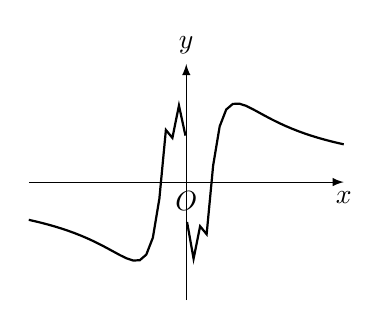
\begin{tikzpicture}
    \draw[-latex](-2,0) -- (2,0) node[below]{$x$};
    \draw[-latex](0,-1.5) -- (0,1.5) node[above]{$y$};
    \filldraw[black] (0,0) node[below]{$O$};
    \draw[black, thick, domain=0.01:2] plot (\x,{sin(pow(\x,-1) r)});
    \draw[black, thick, domain=-2:-0.01] plot (\x,{sin(pow(\x,-1) r)});
\end{tikzpicture}

无穷间断点与振荡间断点都是第二类间断点。

\textcolor{orange}{注意:}两侧邻域都有定义才能讨论间断点问题。

\textbf{例题16:}若$f(x)=\left\{
    \begin{array}{lcl}
        2x+a, & & x\leqslant 0 \\
        e^x(\sin x+\cos x), & & x>0
    \end{array} \right.
$在$(-\infty,+\infty)$内连续,求$a$。

因为连续,所以$f(0)=\lim_{x\to 0^+}f(x)=\lim_{x\to 0^-}f(x)$。

$\therefore a=1$。

\textbf{例题17:}若函数$f(x)=\dfrac{\ln\vert x\vert}{\vert x-1\vert}\sin x$,则x的间断点类型是?

由式子的分式部分可知有两个无定义的间断点:$x=0$,$x=1$。

$\lim_{x\to 1}f(x)=\lim_{x\to 1}\dfrac{x-1}{\vert x-1\vert}\sin x=\left\{
    \begin{array}{lcl}
        x\to 1^+ & \rightarrow & \sin 1 \\
        x\to 1^- & \rightarrow & -\sin 1
    \end{array} \right.
$

所以$x=1$跳跃间断点。

$\lim_{x\to 0}f(x)=\lim_{x\to 0}\ln\vert x\vert\cdot\sin x=\lim_{x\to 0}x\ln\vert x\vert=0$

而$x=0$未定义,所以其为可去间断点。

\end{document}
